\documentclass[12pt]{article}

\usepackage{amsmath, mathtools}
\usepackage{amsfonts}
\usepackage{amssymb}
\usepackage{graphicx}
\usepackage{colortbl}
\usepackage{xr}
\usepackage{hyperref}
\usepackage{longtable}
\usepackage{xfrac}
\usepackage{tabularx}
\usepackage{booktabs}
\usepackage{graphicx}
\usepackage{float}
\usepackage{siunitx}
\usepackage{caption}
\usepackage{pdflscape}
\usepackage{afterpage}
\usepackage{fullpage}
\usepackage{titlesec}
\usepackage[shortlabels]{enumitem}
\usepackage[round]{natbib}
\usepackage{array}

%% Comments

\usepackage{color}

\newif\ifcomments\commentstrue %displays comments
%\newif\ifcomments\commentsfalse %so that comments do not display

\ifcomments
\newcommand{\authornote}[3]{\textcolor{#1}{[#3 ---#2]}}
\newcommand{\todo}[1]{\textcolor{red}{[TODO: #1]}}
\else
\newcommand{\authornote}[3]{}
\newcommand{\todo}[1]{}
\fi

\newcommand{\wss}[1]{\authornote{blue}{SS}{#1}} 
\newcommand{\plt}[1]{\authornote{magenta}{TPLT}{#1}} %For explanation of the template
\newcommand{\an}[1]{\authornote{cyan}{Author}{#1}}

%% Common Parts

\newcommand{\progname}{Chess Connect} % PUT YOUR PROGRAM NAME HERE
\newcommand{\authname}{Team \#4,
\\ Alexander Van Kralingen
\\ Arshdeep Aujla
\\ Jonathan Cels
\\ Joshua Chapman
\\ Rupinder Nagra} % AUTHOR NAMES without MacIDs 

\usepackage{hyperref}
    \hypersetup{colorlinks=true, linkcolor=blue, citecolor=blue, filecolor=blue,
                urlcolor=blue, unicode=false}
    \urlstyle{same}
                                

\graphicspath{{./images/}}

\setcounter{secnumdepth}{4}

\titleformat{\paragraph}
{\normalfont\normalsize\bfseries}{\theparagraph}{1em}{}
\titlespacing*{\paragraph}
{0pt}{3.25ex plus 1ex minus .2ex}{1.5ex plus .2ex}

\begin{document}

\title{Software Requirements Specification for \progname{}: Online tools combined with on-board vision to improve and share your game} 
\author{\authname}
\date{October 4th, 2022}
	
\maketitle

~\newpage

\tableofcontents

~\newpage

\addcontentsline{toc}{section}{Table of Revisions}
\section*{Table of Revisions}
\begin{table}[hp]
\caption{Revision History} \label{TblRevisionHistory}
\begin{tabularx}{\textwidth}{llX}
\toprule
\textbf{Date} & \textbf{Developer(s)} & \textbf{Change}\\
\midrule
2022-10-04 & Jonathan Cels & Template creation and document formatting\\ 
2022-10-04 & Jonathan Cels & Non-functional requirements\\
2022-10-05 & Joshua Chapman & Constants, Monitored Variables, Controlled Variables\\
2022-10-05 & Alexander Van Kralingen & Added Context Diagram\\
2022-10-05 & Joshua Chapman & Problem Description, Assumptions \\
2022-10-05 & Jonathan Cels & Scope, Intended Reader, Stakeholders\\
2022-10-05 & Rupinder Nagra, Jonathan Cels & Functional Requirements\\
2022-10-05 & Arshdeep Aujla & Constraints\\
2022-10-05 & Alexander Van Kralingen & Added Use Cases/Scenarios. Fixed system context diagram position. Added likely change.\\
2022-10-05 & Rupinder Nagra & Purpose, Likely Changes and Unlikely Changes\\
2022-10-05 & Alexander Van Kralingen & Added Undesired Event Handling section and a likely change.\\
2022-10-05 & Arshdeep Aujla & Characteristics of Intended User, Stakeholders\\
2022-10-05 & Arshdeep Aujla & Reflection\\
2022-10-05 & Alexander Van Kralingen & Added FSM\\
2022-10-19 & Jonathan Cels & Added new hazard requirements\\
2022-10-23 & Alexander Van Kralingen & Fixed FSM, added diagram source code\\
2022-11-02 & Jonathan Cels & Changed some NFRs\\
\bottomrule
\end{tabularx}
\end{table}

~\newpage

\section{Units, Terms, Acronyms, and Abbreviations}

\subsection{Table of Units}
Throughout this document SI (Syst\`{e}me International d'Unit\'{e}s) is employed
as the unit system.  In addition to the basic units, several derived units are
used as described below.  For each unit, the symbol is given followed by a
description of the unit and the SI name.

\begin{table}[ht]
  \noindent \begin{tabular}{l l l} 
    \toprule		
    \textbf{symbol} & \textbf{unit} & \textbf{SI}\\
    \midrule 
    \si{\volt} & electric potential & volt\\
    \si{\ampere} & current	& ampere\\
    \si{\ohm} & resistance	& ohm\\
    \si{\second} & time & second\\
    \si{\celsius} & temperature & centigrade\\
    \si{\joule} & energy & joule\\
    \si{\watt} & power & watt (W = \si{\joule\per\second})\\
    \bottomrule
  \end{tabular}
\end{table}

\newpage

\subsection{Abbreviations and Acronyms}
\begin{tabular}{l l} 
  \toprule		
  \textbf{symbol} & \textbf{description}\\
  \midrule 
  A & Assumption\\
  CSA & Canadian Standards Association\\
  DD & Data Definition\\
  FIDE & International Chess Federation or Fédération Internationale des Échecs\\
  GD & General Definition\\
  GS & Goal Statement\\
  IM & Instance Model\\
  LC & Likely Change\\
  LCD & Liquid Crystal Display\\
  LED & Light-Emmitting Diode\\
  MCU & Micro Controller Unit\\
  PS & Physical System Description\\
  R & Requirement\\
  SRS & Software Requirements Specification\\
  SS & Skills for Success\\
  T & Theoretical Model\\
  VnV & Verification and Validation\\
  WCAG & Web Content Accessibility Guidelines\\
  \bottomrule
\end{tabular}\\

\subsection{Mathematical Notation}

\subsection{Terminology and Definitions}
\begin{tabularx}{\linewidth}{ l X }
    \toprule		
    \textbf{Term} & \textbf{Definition}\\
    \midrule 
    Legal Move & Moving a single chess piece from one square on the board to another in a way that follows the rules of chess. \\[0.5cm]
    Resign & To forfeit or surrender a game of chess. \\[0.5cm]
    Draw & To tie a game of chess. \\[0.5cm]
    Draw by Agreement & When both players agree to draw instead of continuing to play. \\[0.5cm]
    Capture & When a piece moves into the space of an opposing piece following the rules of chess, removing that piece from the game. \\[0.5cm]
    Check & A condition that occurs when a player's king is under threat of being captured. \\[0.5cm]
    Checkmate & A condition that occurs when a player's king is in check \textbf{and} has no legal moves to escape. 
    This ends the game, and the player who delivered the checkmate wins. \\[0.5cm]
    Stalemate & A type of draw that occurs when the king is \textbf{not} in check, but no piece can be moved without putting the king in check. \\[0.5cm]
    \bottomrule
  \end{tabularx}

\section{Introduction}
\subsection{Document Purpose}
The purpose of this document is to provide a set of requirements for a system that will integrate over-the-board chess with the online world of chess to assist in learning the game in a flexible manner.
This includes a detailed description of our functional and non-functional requirements, including the performance and attributes of our design. 
The document also includes a project overview showcasing the behaviour with event handling and system diagrams, and the likely and unlikely changes we expect to 
encounter throughout the development of our product.

\subsection{Characteristics of Intended Reader}
{The document is written with the purpose of guiding development for the \progname{} team. The intended readers of this document 
are the developers of \progname{}, Dr.~Spencer Smith, and Nicholas Annable, the teaching assistant assigned to this project. The 
document is thus written for an audience that is well-versed in formal specification at a university level. This includes models, 
diagrams, and mathematical notation. Readers should also have a university-level understanding of electrical circuit knowledge.}

\subsection{Characteristics of Intended User}
{This project will assist chess players of any level that are looking for a tool to help them learn and study the game. For beginners, 
the board serves as a learning tutorial and a general introduction to the game, while intermediate and advanced players can use the 
engine move recommendations to study new lines, puzzles, and specific positions to enhance their chess skills.}

\subsection{Stakeholders}
{The professor and TAs for the course SFWRENG 4G06 as they will be providing the feedback which will directly affect the project’s development. 
Society is also a stakeholder because this project will provide the members of society another gateway to be involved in the community through the game of chess. Lastly, this project will 
also be relevant to chess tournament organizers looking for a method to easily broadcast and share their games online in real-time.}

\section{Problem Description}

{Online chess has functionality for both beginners and experienced players to
learn and practice the game. However, these forms of learning emphasize a
visual style of learning using a standard keyboard and mouse, while physical
boards place emphasis on tactile learning when learning or studying the game.
The highest-rated chess players often use a combination of the two styles to
optimize their play. However, no option exists for players of any skill level to
integrate their over-the-board and online play with one solution.\\
Chess Connect plans to centralize these two mediums of studying the game in
order to provide flexibility and remove constraints for new players in learning
how to play chess.}


\section{Assumptions}

\begin{enumerate}[{A}1., leftmargin=2\parindent]
    \item Users of the board have knowledge of the starting positions and will
    set them up before the start of a new game.  \\
    \item Users will not make illegal moves outside of beginner mode. \\
    \item Game termination as dictated by the rules of chess \cite{RulesofChess} \\
    \item {During gameplay, users will not take back moves. When a piece is placed
    on the board, that move is final.} \\
    \item Users will have the knowledge of bluetooth setup and connection. \\
\end{enumerate}

\section{Constraints}

\begin{table}[H]
  \centering
      \setlength{\leftmargini}{0.4cm}
      \begin{tabular}{| >{\centering\arraybackslash}m{3cm} | 
        >{\centering\arraybackslash}m{12cm} |}
      \hline
      \rowcolor[gray]{0.9}
      C1 & The cost should not exceed CAD \$750\\
      \hline 
      Rationale & This is the maximum budget alloted to this project as per the course requirements.\\
      \hline 
      \end{tabular}
  \label{Table}
  \end{table}
  
\begin{table}[H]
  \centering
      \setlength{\leftmargini}{0.4cm}
      \begin{tabular}{| >{\centering\arraybackslash}m{3cm} | 
        >{\centering\arraybackslash}m{12cm} |}
      \hline
      \rowcolor[gray]{0.9}
      C2 & The project must be completed by the winter semester of 2023\\
      \hline 
      Rationale & This is the allocated time for this project as per the course requirements.\\
      \hline 
      \end{tabular}
  \label{Table}
  \end{table}  

\section{Scope}
{The system is called \progname{}, and will include a software application and physical hardware device. The hardware will take the 
form of a chess set, and will collect and relay move and piece data. The device will convey the best moves for the specific board 
position, and will convey legal moves for specific pieces.The device will be connected to the software application, relaying and 
receiving relevant data. The software application will model and track the physical device, and will broadcast the data in an accessible 
format. The application will be constrained to a 2-dimensional model of the hardware device, showing a top-down view of the game.}

\bigskip
\noindent{\textbf{In-scope} items for the system include the following:
\begin{enumerate}
    \item Modeling and tracking a chess game played using the \progname{} hardware
    \item Displaying and broadcasting the game state on the \progname{} software application
    \item Giving users an option to choose between beginner mode, engine mode, and normal mode
    \begin{itemize}
        \item Beginner mode will display legal moves for individual pieces when a chess piece is picked up, and will warn the players when an illegal move is made
        \item Engine mode will display the best moves as determined by a chess engine for the position
        \item Normal mode will disable the engine and beginner mode features. This is intended for regular play between experienced players
    \end{itemize}
\end{enumerate}}

\bigskip

\noindent{The following items are deemed to be \textbf{out of scope}:
\begin{enumerate}
    \item FIDE (International Chess Federation) standards for tournament appropriate chess equipment
    \item Tracking and support for alternate chess variants such as Chess960, Atomic Chess, King of the Hill. More information found here: \cite{ListOfChessVariants2022}.
    \item Proper tracking of alternate starting positions like puzzles
    \item Proper tracking of illegal moves and rule violations when warnings are ignored
\end{enumerate}}

\section{Project Overview}
\subsection{System Context Diagram}{

    The context of the system invloves two integrated but separate system components, as well as two distinct end users.

\begin{figure}[H]
  \begin{center}
    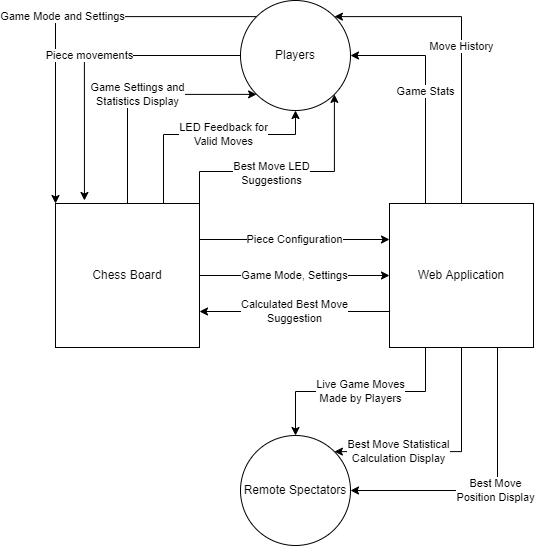
\includegraphics[scale=0.65]{chess-connect-system-context.png}
    \caption{Overall System Context}
    \label{Fig_SystemContext} 
  \end{center}
\end{figure}

\subsection{Behaviour Overview}
\begin{figure}[H]
    \begin{center}
      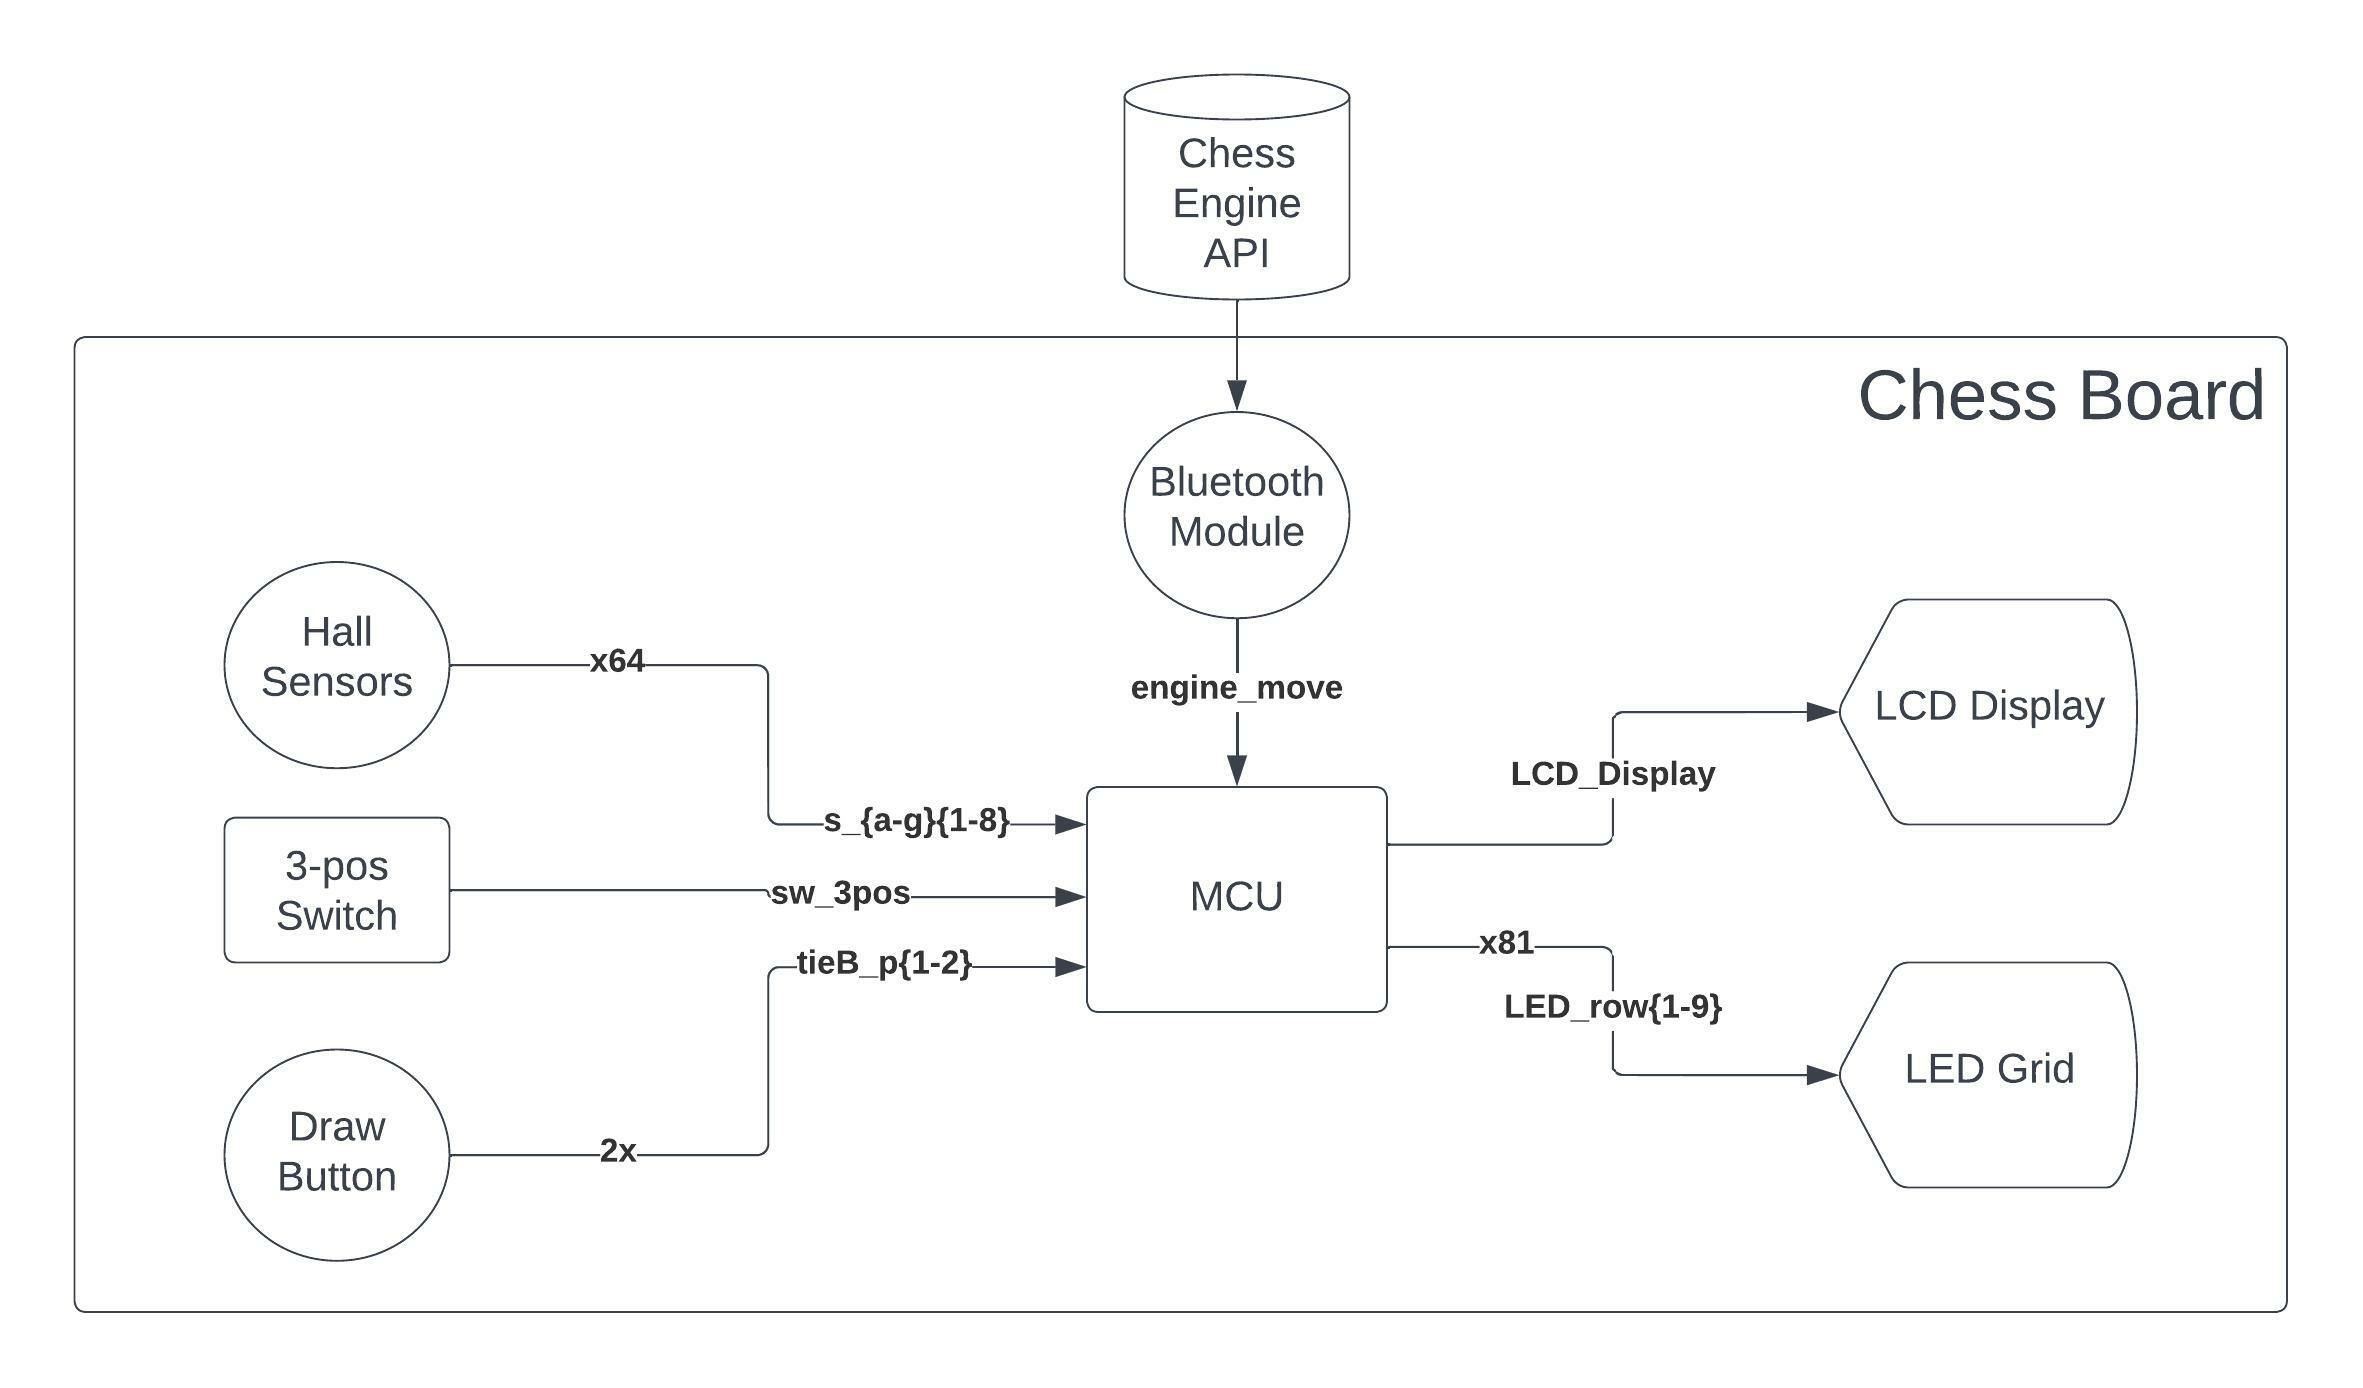
\includegraphics[scale=0.8]{Hardware_System_Context_Diagram.jpeg}
      \caption{On-board System Context}
      \label{Fig_SystemContext2} 
    \end{center}
  \end{figure}

\subsection{Normal Operation}
\subsubsection{Description}{
    The normal operation of the chess board involves configuring game mode and settings, reading the physical positions and identifiers (magnetic strength) of the pieces, 
    lighting up corresponding LEDs and determining legal moves on the micro-controller. There will be three game modes: Normal Mode (no LED feedback), Engine Mode (best moves 
    calculated by a chess engine and displayed by an LCD display) and Beginner Mode (legal moves displayed by LED when a piece is picked up). The micro-controller will also be 
    simultaneously transmitting data to the server via Bluetooth and receiving responses in the form of ``best'' moves from the server. The server will be calculating these 
    best moves in real time depending on the configuration of the pieces on the board sent from the chess board, and sending it back over Bluetooth every time it is queried
    while the game is in ``Engine Mode''. The server will also be communicating all of this information to a web application where users can tune in and watch the pieces and see
    game stats in real time.
}

\subsubsection{Finite State Machine}{
\begin{figure}[H]
    \begin{center}
      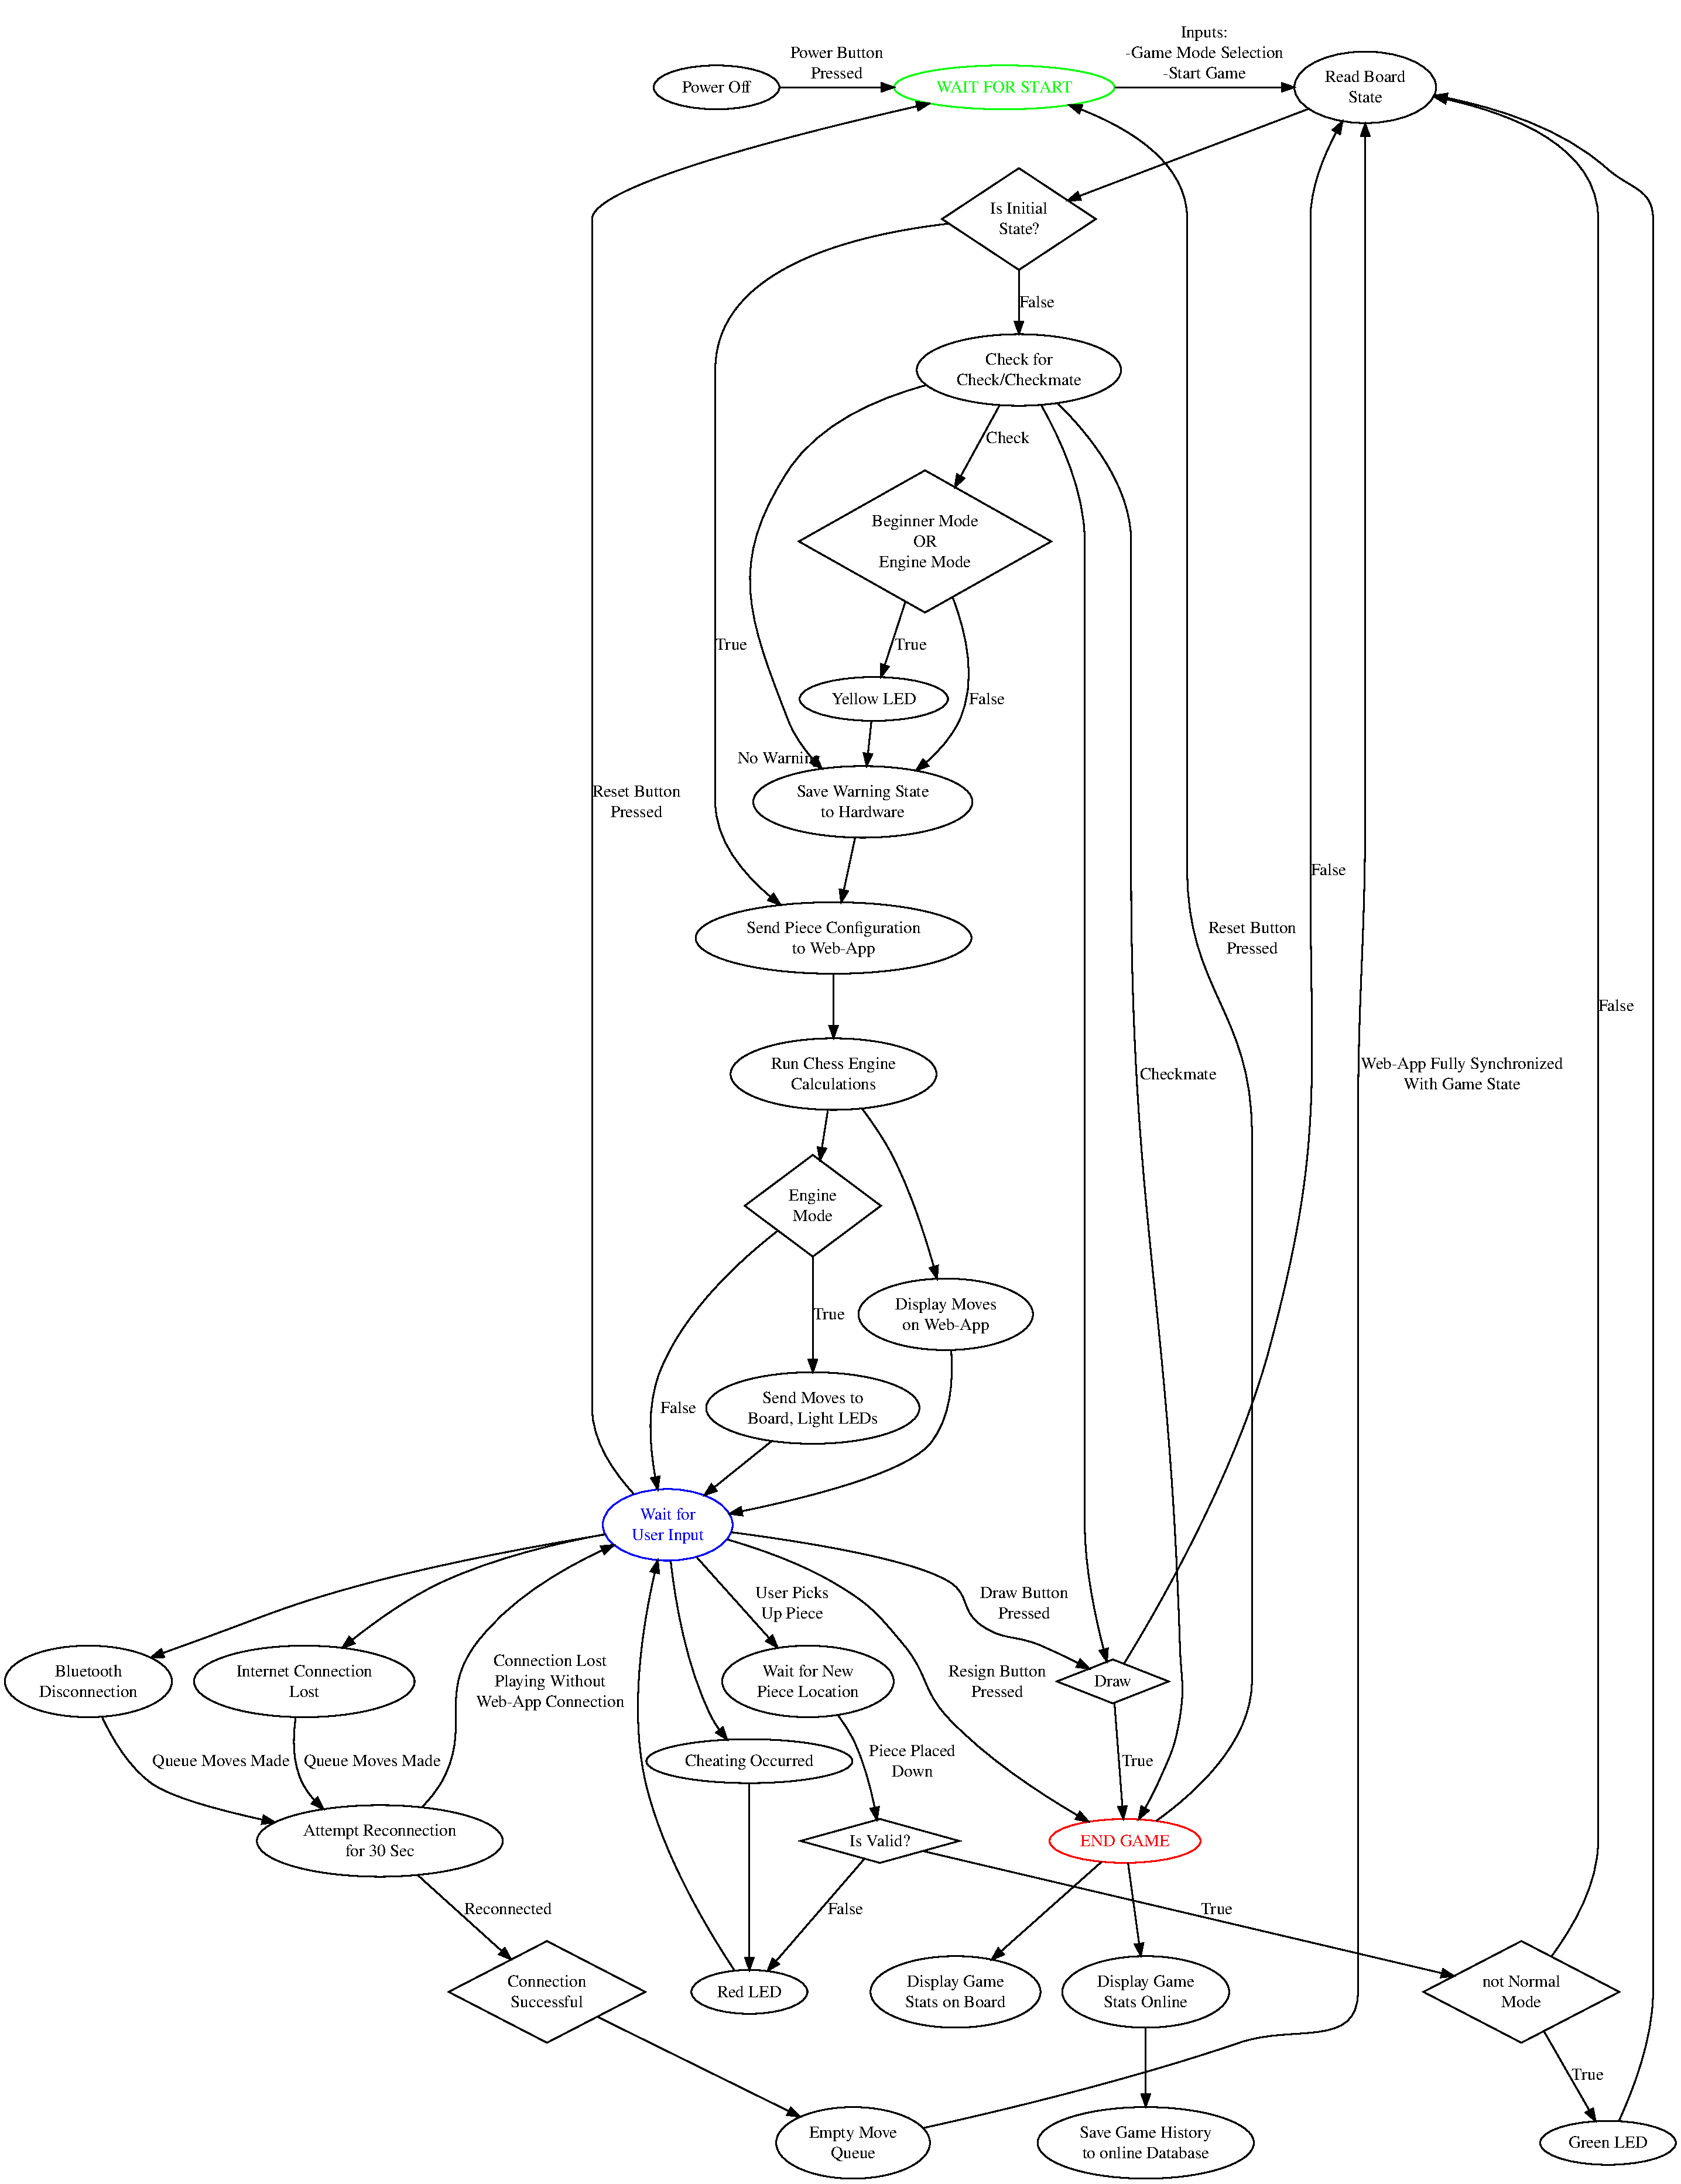
\includegraphics[scale=0.30]{chess-connect-FSM.pdf}
      \caption{Finite State Machine Detailing Normal System Behaviour. Green indicates initial state, blue indicates waiting for user input and red indicates end state.}
      \label{Fig_FSM} 
    \end{center}
  \end{figure}
}

\subsubsection{Use Cases/Scenarios}{
    
    \paragraph{Normal Mode}{
        Users play the game without any LED feedback. This would typically be a formal match involving players that are familiar with the game. Moves would still be broadcast to the
        web application, and move history will still be recorded for future reference.
    }
        
    \paragraph{Engine Mode}{
        Users play the game with LCD feedback indicating which pieces to move to which positions that would be statistically the most probable move to win the game. This game mode would
        be most likely played as a way to improve one's skill level and to gain a deeper understanding of the game.
    }
    
    \paragraph{Beginner Mode}{
        Users play the game with LED feedback on lifting a piece. The piece lifted will be determiend by the hardware and corresponding legal moves will be lit up on the board. This game
        mode is designed to help beginners learn the game of chess. Legal moves will involve more complex strategies such as ``en passant'' and ``castling''.
    }
        
    \paragraph{Studying Past Games}{
        The web application will have a record of the moves made in past games. This can be used to study the game moves and understand scenarios which could have been handled differently
        to produce a more favourable outcome.
    }
    
    \paragraph{Tournament Play}{
        Since the moves made in the game will be broadcasted live to the internet via the web application, tournaments can be held with spectators watching the game in real time.
    }
}

\subsection{Undesired Scenario Handling}{
    \paragraph{Earthquake Scenario}{
        Also known as the ``sore loser scenario'', when some or all of the pieces are removed from their spaces within a short amount of time, the game will be ended as a draw. 
    }
    
    \paragraph{Power Loss}{
        When the power to the board is cut, the web application will end the game as a draw. The board will also have to be reconfigured back into the default starting positions for all pieces.
    }
    
    \paragraph{Bluetooth Disconnection}{
        On bluetooth disconnection, the board will attempt to reconnect for 30 seconds. Upon the expiration of this timer, the game will end as a draw.
    }
    
    \paragraph{Internet Disconnection}{
        On internet disconnection, the server will keep a history of past moves made. On reconnection, the game will be updated to reflect these moves as they are sent through the
        queue to the hosted interface.
    }
    
    \paragraph{Cheating}{
        If pieces are moved or removed out of turn, the spaces which were affected will be lit up with red LEDs. When the board is returned to the state before cheating occurred,
        the game will resume as normal.
    }
    
}

\section{System Level Variables}
\subsection{Constants}

\begin{table}[H]
  \centering
      \setlength{\leftmargini}{0.4cm}
      \begin{tabular}{| >{\centering\arraybackslash}m{5cm} | 
        >{\centering\arraybackslash}m{2cm} | 
        >{\centering\arraybackslash}m{5cm} |}
      \hline
      \rowcolor[gray]{0.9}
      Constant & Unit & Value\\
      \hline
      Chess board width & inches & 12\\
     \hline
     Chess board length & inches & 12\\
     \hline
     Chess board tile width & inches & 1.5\\
     \hline 
     Chess board tile length & inches & 1.5\\ 
     \hline 
     Supply Power to Board & Volts & 110 VAC\\
     \hline
      \end{tabular}
  \label{Table}
  \end{table}

\subsection{Monitored Variables}

\begin{table}[H]
  \centering
      \setlength{\leftmargini}{0.4cm}
      \begin{tabular}{| >{\centering\arraybackslash}m{2.5cm} | 
        >{\centering\arraybackslash}m{2cm} | 
        >{\centering\arraybackslash}m{9cm} |}
      \hline
      \rowcolor[gray]{0.9}
      Variable & Units & Description\\
      \hline
      s\_a\{1-8\} & Volts & States of tiles a1 - a8 on the board. They are analog signals 
      converted to digital and the state of the tile is determined. The possible states of 
      each tile is empty, black/white pawn, black/white rook, black/white knight, 
      black/white bishop, black/white queen, black/white king. \\
      \hline
      s\_b\{1-8\} & Volts & States of tiles b1 - b8 on the board. " " \\
      \hline
      s\_c\{1-8\} & Volts & States of tiles c1 - c8 on the board. " " \\
      \hline
      s\_d\{1-8\} & Volts & States of tiles d1 - d8 on the board. " " \\
      \hline
      s\_e\{1-8\} & Volts & States of tiles e1 - e8 on the board. " " \\
      \hline
      s\_f\{1-8\} & Volts & States of tiles f1 - f8 on the board. " " \\
      \hline
      s\_g\{1-8\} & Volts & States of tiles g1 - g8 on the board. " " \\
      \hline
      sw\_3pos & Volts & The three-position switch is located
      on top of the board. It toggles between the beginner 
      advice, engine advice and normal modes.\\
      \hline
      tieB\_p\{1-2\} & Volts & The ``draw'' push-button for each player is located on 
      the top of the board on their respective sides. When both players press their button
      the game is a draw. \\
      \hline
      engine\_move & chess notation & The chess engine API provides best moves into 
      the system. \\
      \hline 
      \end{tabular}
  \label{Table}
  \end{table}

\subsection{Controlled Variables}

\begin{table}[H]
  \centering
      \setlength{\leftmargini}{0.4cm}
      \begin{tabular}{| >{\centering\arraybackslash}m{3cm} | 
        >{\centering\arraybackslash}m{2cm} | 
        >{\centering\arraybackslash}m{9cm} |}
      \hline
      \rowcolor[gray]{0.9}
      Variable & Units & Description\\
      \hline 
      LED\_row\{1-9\} & Volts & A total of 81 LEDS will be located under the board. They 
      are on the corner of each tile and illuminate based on conditions of the inputs. \\
      \hline 
      LCD\_Display & Volts & An LCD Display is located on the chess board to indicate
      best moves delivered by the engine. \\
      \hline 
      \end{tabular}
  \label{Table}
  \end{table}


\section{Requirements}
\subsection{Functional Requirements}
{The system has two states, the Game Active State and the Game Inactive State. When in the Game Active State, the system can be in one of three possible ``user modes''. The user modes are Normal Mode, Engine Mode, and Beginner Mode.}

\begin{figure}[h]
    \begin{center}
        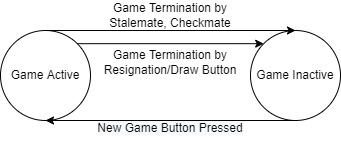
\includegraphics[scale=0.75]{GameActiveFSM.drawio}
        \caption{Game State Diagram}
        \label{Fig_GameStates} 
    \end{center}
\end{figure}

\subsubsection{Game Active State}
\paragraph{Chess Board}
\begin{enumerate}[{GA}1., leftmargin=2\parindent]
    \item Pressing the Resign/Draw button will change the system to the Game Inactive State.
    \item Pressing the New Game button will have no effect.
    \item Allow users to switch between user modes, choosing Normal Mode, Engine Mode, or Beginner Mode by using the User Mode switch on the side of the board.
    \item The chess board follows the \textbf{Chess Board} section for the respective user mode being played.
\end{enumerate}

\paragraph{Data Transfer}
\begin{enumerate}[{GA}1., leftmargin=2\parindent, resume]
    \item Data transfer follows the \textbf{Data Transfer} section for the respective user mode being played.
\end{enumerate}

\paragraph{Web Application}
\begin{enumerate}[{GA}1., leftmargin=2\parindent, resume]
    \item Entering the Game Active State will reset the game state to the starting position.
    \item Game termination of type stalemate or checkmate shall change the system to the Game Inactive State.
    \item The web application follows the \textbf{Web Application} section for the respective user mode being played.
\end{enumerate}

\subsubsection{Game Inactive State}
\paragraph{Chess Board}
\begin{enumerate}[{GI}1., leftmargin=2\parindent]
    \item Pressing the New Game button will change the system to the Game Active State.
    \item Using the User Mode switch at the side of the board will have no effect until the system is in the Game Active State.
    \item Pressing the Resign/Draw button will have no effect.
\end{enumerate}

\paragraph{Data Transfer}
\begin{enumerate}[{GI}1., leftmargin=2\parindent, resume]
    \item The board state data is not sent to the web application when a piece is moved.
\end{enumerate}

\paragraph{Web Application}
\begin{enumerate}[{GI}1., leftmargin=2\parindent, resume]
    \item The web application will display the final game state upon game termination.
    \item The web application will display a message with the game termination type (stalemate, checkmate, resignation, draw).
\end{enumerate}

\subsubsection{Normal Mode}
\paragraph{Chess Board}
\begin{enumerate}[{NB}1., leftmargin=2\parindent]
    \item The system shall store the position, colour, and type of the previously moved piece in the micro-controller.
    \item Allow each player the ability to resign by holding down the Resign/Draw button for ENDTIME seconds located on their side of the board.
    \item Allow the players the ability to draw by having them both hold down the Resign/Draw button for ENDTIME seconds located on their side of the board. 
\end{enumerate}

\paragraph{Data Transfer}
\begin{enumerate}[{ND}1., leftmargin=2\parindent]
    \item The system shall send the micro-controller output over the chosen data transfer method as an input to the web application.
\end{enumerate}

\paragraph{Web Application}
\begin{enumerate}[{NA}1., leftmargin=2\parindent]
    \item The web application will receive data related to the previous move.
    \item The web application will display the updated game board configuration with the data of the previous move.
    \item In event of game termination (stalemate, checkmate, resignation, draw), the web application will display a message with the method of game termination. The system shall change to the Game Inactive State.
\end{enumerate}

\subsubsection{Engine Mode}
\paragraph{Chess Board}
\begin{enumerate}[{EB}1., leftmargin=2\parindent]
    \item The system shall store the position, colour, and type of the previously moved piece in the micro-controller.
    \item Allow each player the ability to resign by holding down the Resign/Draw button for ENDTIME seconds located on their side of the board.
    \item Allow the players the ability to draw by having them both hold down the Resign/Draw button for ENDTIME seconds located on their side of the board.
    \item The system shall show the top engine moves on the LCD display.
\end{enumerate}

\paragraph{Data Transfer}
\begin{enumerate}[{ED}1., leftmargin=2\parindent]
    \item The system shall send the micro-controller output over the chosen data transfer method as an input to the web application.
    \item The system shall send the web application engine moves to the LCD display over the chosen data transfer method.
\end{enumerate}

\paragraph{Web Application}
\begin{enumerate}[{EA}1., leftmargin=2\parindent]
    \item The web application will receive data related to the previous move.
    \item The web application will display the updated game board configuration with the data of the previous move.
    \item The system shall input the current chess game position to a chess engine.
    \item The system shall use the chess engine to evaluate the position and calculate the best engine moves.
    \item The system shall display the calculated engine moves on the web application.
    \item In event of game termination (stalemate, checkmate, resignation, draw), the web application will display a message with the method of game termination. The system shall change to the Game Inactive State.
\end{enumerate}

\subsubsection{Beginner Mode}
\paragraph{Chess Board}
\begin{enumerate}[{BB}1., leftmargin=2\parindent]
    \item The system shall store the position, colour, and type of the previously moved piece in the micro-controller.
    \item When a user picks up a piece, allow them to view all legal moves with green LED lights on valid squares.
    \item If an illegal move is made, the tile that the piece is moved onto will display a red LED light.
    \item Allow each player the ability to resign by holding down the Resign/Draw button for ENDTIME seconds located on their side of the board.
    \item Allow the players the ability to draw by having them both hold down the Resign/Draw button for ENDTIME seconds located on their side of the board.
\end{enumerate}

\paragraph{Data Transfer}
\begin{enumerate}[{BD}1., leftmargin=2\parindent]
    \item The system shall send the micro-controller output over the chosen data transfer method as an input to the web application.
\end{enumerate}

\paragraph{Web Application}
\begin{enumerate}[{BA}1., leftmargin=2\parindent]
    \item Allow user to view instructions regarding the rules of chess on web application.
    \item The web application will display the updated game board configuration with the data of the previous move.
\end{enumerate}



\subsection{Nonfunctional Requirements}

\newcounter{vnvSectionNfr}
\setcounter{vnvSectionNfr}{1}

\newcounter{nfrNum}
\setcounter{nfrNum}{1}

\subsubsection{Look and Feel Requirements}
\label{NFR_LF}
\paragraph{Appearance Requirements}
\begin{enumerate}[{LF}1., leftmargin=2\parindent]
    \item The product shall use white, black, grey, and brown as its primary colours.
    \item The product shall use green, red, and blue as its secondary colours.
\end{enumerate}

\paragraph{Style Requirements}
\begin{enumerate}[{LF}1., leftmargin=2\parindent, resume]
    \item The product shall look and feel similar enough to traditional chess boards and chess pieces that the target audience will 
    recognize the product as a chess set when encountering it for the first time. The level and speed of audience recognition achieved 
    by the design shall be described following the procedure given in Section 5.2.\thevnvSectionNfr\stepcounter{vnvSectionNfr}~of the VnV 
    (Verification and Validation) Plan.
\end{enumerate}



\subsubsection{Usability and Humanity Requirements}
\label{NFR_UH}
\paragraph{Ease of Use Requirements}
\begin{enumerate}[{UH}1., leftmargin=2\parindent]
    \item The system shall require the user to place chess pieces fully on their intended squares.
    \item Physical hardware components of the system will not impede the user during play.
\end{enumerate}

\paragraph{Personalization and Internationalization Requirements}
\begin{enumerate}[{UH}1., leftmargin=2\parindent, resume]
    \item The system will only display information in English.
    \item The system will only use the Arabic numerals.
\end{enumerate}

\paragraph{Learning Requirements}
\begin{enumerate}[{UH}1., leftmargin=2\parindent, resume]
    \item The product shall be able to be used by members of the public over with no previous training. Details on the learnability 
    of the system shall be described following the procedure given in Section 5.2.\thevnvSectionNfr\stepcounter{vnvSectionNfr}
    of the VnV Plan.
\end{enumerate}

\paragraph{Understandability and Politeness Requirements}
\begin{enumerate}[{UH}1., leftmargin=2\parindent, resume]
    \item All symbols and words shall be similar to historically used Chess symbols. \cite{ChessHistory2003}
\end{enumerate}

\paragraph{Accessibility Requirements}
\begin{enumerate}[{UH}1., leftmargin=2\parindent, resume]
    \item The system shall follow guidelines for correct size and colour contrast ratio for text to the background as stated in the \cite{WCAG2018}.
\end{enumerate}



\subsubsection{Performance Requirements}
\label{NFR_PR}
\paragraph{Speed and Latency Requirements}
\begin{enumerate}[{PR}1., leftmargin=2\parindent]
    \item The average time between a user placing down a piece and the visual model response shall be small.
    \item The maximum time between a user placing down a piece and the visual model response shall be small.
    \item The average time between a user picking up a piece and the visual board indicator response shall be small.
    \item The maximum time between a user picking up a piece and the visual board indicator response shall be small. 
    The degree of speed for PR1 through PR4 shall be described following the procedure given in Section 5.2.\thevnvSectionNfr\stepcounter{vnvSectionNfr}
    of the VnV Plan.
\end{enumerate}

%Modified from Safety-Critical Requirements to better cover the SRS rubric
\paragraph{Health and Safety-Critical Requirements}
\begin{enumerate}[{PR}1., leftmargin=2\parindent, resume]
    \item The system shall be properly grounded according to the Canadian Electrical Code. \cite{CanadianElectricalCode2021}
    \item The maximum power on any single wire shall be within the safety limits described in the Canadian Electrical Code.
\end{enumerate}

\paragraph{Precision or Accuracy Requirements}
\begin{enumerate}[{PR}1., leftmargin=2\parindent, resume]
    \item The software application game state will model the game state on the \progname{} hardware with a high degree of accuracy. 
    The level of accuracy shall be described following the procedure given in Section 5.2.\thevnvSectionNfr\stepcounter{vnvSectionNfr}
    of the VnV Plan.
\end{enumerate}

\paragraph{Reliability and Availability Requirements}
\begin{enumerate}[{PR}1., leftmargin=2\parindent, resume]
    \item The product shall be available with a minimum of 95\% uptime. 
\end{enumerate}

\paragraph{Robustness or Fault-Tolerance Requirements}
\begin{enumerate}[{PR}1., leftmargin=2\parindent, resume]
    \item The software application shall maintain the game state if the connection between the software and hardware systems is interrupted.
\end{enumerate}

\paragraph{Capacity Requirements}
\begin{enumerate}[{PR}1., leftmargin=2\parindent, resume]
    \item The software shall require computer memory to function effectively. The level of memory capacity required shall be described following
    the procedure given in Section 5.2.\thevnvSectionNfr\stepcounter{vnvSectionNfr} of the VnV Plan.
\end{enumerate}

\paragraph{Scalability or Extensibility Requirements}
\begin{enumerate}[{PR}1., leftmargin=2\parindent, resume]
    \item The product must support the addition of new features and components.
\end{enumerate}

\paragraph{Longevity Requirements}
\begin{enumerate}[{PR}1., leftmargin=2\parindent, resume]
    \item The product must be supported while the application remains deployed.
    \item The product will depend on the continued support of packages and libraries.
\end{enumerate}



\subsubsection{Operational and Environmental Requirements}
\label{NFR_OE}
\paragraph{Expected Physical Environment}
\begin{enumerate}[{OE}1., leftmargin=2\parindent]
    \item The hardware and software systems shall be close enough to each other to facilitate communication. The degree of proximity required 
    will be 20 meters or less.
    \item The area shall be clear of potentially dangerous or harmful environmental factors.
\end{enumerate}

\paragraph{Requirements for Interfacing with Adjacent Systems}
\begin{enumerate}[{OE}1., leftmargin=2\parindent, resume]
    \item The system shall interface with an external server to make requests to a chess engine.
\end{enumerate}

\paragraph{Productization Requirements}
\begin{enumerate}[{OE}1., leftmargin=2\parindent, resume]
    \item The product shall be deployed to a public website where users may access it.
\end{enumerate}

\paragraph{Release Requirements}
\begin{enumerate}[{OE}1., leftmargin=2\parindent, resume]
    \item The product will be tested for bugs and issues. These issues will be fixed and the application will be redeployed accordingly.
\end{enumerate}



\subsubsection{Maintainability and Support Requirements}
\label{NFR_MS}
\paragraph{Maintenance Requirements}
\begin{enumerate}[{MS}1., leftmargin=2\parindent]
    \item The product shall be maintained actively by the developers until the \progname{} team graduates.
\end{enumerate}

\paragraph{Supportability Requirements}
N/A

\paragraph{Adaptability Requirements}
\begin{enumerate}[{MS}1., leftmargin=2\parindent, resume]
    \item The software application will be able to be hosted on Apple, Windows, and Linux devices.
    \item The product shall be accessible from any web browser.
\end{enumerate}



\subsubsection{Security Requirements}
\label{NFR_SR}
\paragraph{Access Requirements}
\begin{enumerate}[{SR}1., leftmargin=2\parindent]
    \item Only the \progname{} team are able to modify the software system.
\end{enumerate}

\paragraph{Integrity Requirements}
\begin{enumerate}[{SR}1., leftmargin=2\parindent, resume]
    \item The product will not store game data after a game has concluded.
    \item The system shall locally maintain the current game state, making no changes until a connection is restablished.
    \item The system shall alert the user that a connection has been lost.
    \item The system shall prompt the user to take an appropriate hazard-specific action.
\end{enumerate}

\paragraph{Privacy Requirements}
\begin{enumerate}[{SR}1., leftmargin=2\parindent, resume]
    \item The product will not store or collect user data.
\end{enumerate}

\paragraph{Audit Requirements}
\begin{enumerate}[{SR}1., leftmargin=2\parindent, resume]
    \item Requirements shall be easy to follow and verify against both the system and the VnV plan in order to facilitate regular inspections.
\end{enumerate}

\paragraph{Immunity Requirements}
N/A



\subsubsection{Political and Cultural Requirements}
\label{NFR_PC}
\paragraph{Cultural Requirements}
\begin{enumerate}[{PC}1., leftmargin=2\parindent]
    \item The product will not use and terms or symbols that are deemed offensive to any culture.
\end{enumerate}

\paragraph{Political Requirements}
N/A



\subsubsection{Legal Requirements}
\label{NFR_Legal}
\paragraph{Compliance Requirements}
\begin{enumerate}[{LR}1., leftmargin=2\parindent]
    \item The system shall comply with the Canadian Electrical Code \cite{CanadianElectricalCode2021}.
\end{enumerate}

\paragraph{Standards Requirements}
\begin{enumerate}[{LR}1., leftmargin=2\parindent, resume]
    \item The product shall follow \cite{WCAG2018}.
\end{enumerate}


\section{Likely Changes}
\noindent
\begin{enumerate}[{LC}1., leftmargin=2\parindent]
    \item Reviewing past games allows players to evaluate their own positions with a better understanding on how to play in future games.
    We will use databases such as MySQL and MongoDB in order to store these games for users to view.
    \item An additional user mode, Study Mode, that will allow users to set up puzzles that do not start from the default position.
    It will allow users to practice a specific phase of the game, including the ability to take back moves without having to play out a full game with an opponent. 
    This mode is meant to be used individually, also allowing a user to use and study the board without the necessity of another player.
    \item Online chess has extensive communities on existing platforms. To promote code reusability, the Chess Connect online platform will interface with popular existing websites.
    Users of the board have the capability to share their games with a larger community via these platforms in addition to the custom web application. These sites include, but are not limited to, Chess.com and Lichess.
    \item An additional game setting to enable either white or black to be a ``computer'' opponent will be implemented in Engine Mode. The user will be able to set a skill level
    for the computer, and moves will be displayed as squares lit up by the on-board LEDs.
    \item The backend/database programming languages and frameworks previously listed
    are subject to change depending on the use of the data transfer functionality, in which comptibility to the hardware would play a role
    in picking our technology stack.  
    \item The load capacity of our system is initially set low for the
    first edition of this application. As demand for the application increases, the load capacity must also increase to support a
    larger user base.
    \item The method of data transfer is subject to change depending on
    interfacing between the hardware and software. Examples of these are Bluetooth and USB connected to the board.
    \item The dimensions of the chess board are subject to change based
    the 3D-printed designs we use for the pieces. 
    \item When pieces are lost, power is cut or data transmission is cut, the current result is ending the game as a draw. Adding the ability for the board to start from any state
    would allow the players to resume from where they left off. This would require several other options such as ``which colour starts'', ``pausing the game'' and ``resume from
    last saved configuration''.
\end{enumerate}
  
\section{Unlikely Changes}    
\noindent
\begin{enumerate}[{UC}1., leftmargin=2\parindent]
    \item Since overarching idea of the project is integration between
    over the board and online chess, a web application will be necessary.
    \item There must be sensors to locate the pieces in order to solve tracking and object detection.
    \item The most popular and easy to use chess engine is Stockfish, which is 
    open source and includes a well-written API documentation. This will likely be the engine we will be using for predicting future moves.
    \item As a learning application, giving beginners the ability to learn quickly
    is a big priority, so the application will include a beginner mode to help familiarize players with the movement of the chess pieces.
    \item Although the back-end/database technologies are subject to change,
    the front-end will make use of our past members' experience in user interface design. For this reason, the technologies
    previously mentioned for front-end are unlikely to change.
\end{enumerate}

\section{Traceability Matrix}

\begin{table}[H]
    \centering
        \setlength{\leftmargini}{0.4cm}
        \begin{tabularx}{\linewidth}{|c|X|}
        \hline
        A1 & GI1 \\
        \hline 
        A2 & BB3 \\ 
        \hline 
        A3 & BB2, BB3 \\
        \hline
        A4 & UH1 \\
        \hline
        BA1 & UH5 \\
        \hline
        7.3.2.1 & NB1,  NB2,  NB3,  ND1, NA1, NA3, \\
        \hline 
        7.3.2.2 & EB1, EB2, EB3, EB4 ED1, ED2, EA1, EA2, EA3, EA4, EA5, EA6\\
        \hline
        7.3.2.3 & BB1, BB2, BB3, BB4, BB5, BD1, BA1, BA2 \\
        \hline
        7.4.0.4 & PR9\\ 
        \hline
        7.4.0.5 & PR9\\
        \hline
        PR11 & LC1, LC2, LC3, LC4, LC5, LC6, LC7, LC8, LC9 \\
        \hline
        LF2 & BB2, BB3 \\ 
        \hline
        \end{tabularx}
    \label{Table}
    \end{table}
  
  

\appendix
\section{Reflection}

\subsection{Skills for Success and Learning Approaches}
\noindent
\begin{enumerate}[{SS}1., leftmargin=2\parindent]
    \item Proper unit tests must be created for the integration between the web application
     and micro-controller. The web application will be made using React so this a skill 
     that will have to be learned. React is a popular front-end framework that encompasses all of the core front-end technologies such as
     HTML, CSS, and Javascript. This required knowledge will be acquired by reading 
     documentation and studying open-source projects. This will be done by group members Jonathan Cels, Rupinder Nagra, and Alexander Van Kralingen.
    \item The back-end system will likely be created using Python and its related frameworks, which is a popular setup for back-end stacks
    in the field of web development. It will also be useful to acquire knowledge in relational and non-relational databases such as MySQL
    and MongoDB. These skills will have to be learned by also reading online documentation and blog forums. This will be done by Rupinder Nagra.
    \item Continuous integration/deployment will have to be used in the project. These skills will be learned by reviewing the tutorials related to this topic as well as reading online documentation. This will be done by member Alexander Van Kralingen.
    \item The micro-controller will need to be set up to use Bluetooth to communicate between the web application and the micro-controller. This will be learned by reading the documentation for the Bluetooth hardware chosen. The skills required for this will be learned by members Jonathan Cels, Joshua Chapman, and Alexander Van Kralingen.
    \item The micro-controller will need to be programmed with the rules of chess. The rules of chess can be found through online resources, with various packages and libraries also able to implement them. This will be done by member Joshua Chapman.
    \item Utilisation of a Hall sensors to identify unique chess pieces using magnets is required. Knowledge of installing and soldering hardware components will have to be learned. This knowledge will be acquired by reading blog posts by people who have used these components and watching tutorial videos on media platforms such as YouTube. This will be done by member Arshdeep Aujla and Joshua Chapman.
    \item The relation between the inputs and outputs will have to be mapped using Karnaugh Maps and State Machine Tables. This will be learned by reviewing related course materials from previous/current years. This will be done by member Arshdeep Aujla.
\end{enumerate}
\newpage

\bibliographystyle {plainnat}
\bibliography {../../refs/References}
\end{document}